\section{Outils de gestion de projet}

\subsection{Méthodes agiles}

Pour réaliser ce projet, nous avons choisi de faire de l'Agile, avec la méthode SCRUM. Nous nous sommes principalement servi des cours de gestion de projet de ce semestre, en particulier des interventions de Sandrine Maton. Faire de l'Agile permet d'avoir un rendu fonctionnel à chaque fin de sprint, et donc de s'assurer d'avoir un rendu final. De plus, c'est une manière de faire qui se dévellope en entreprise, nous voulions donc l'expérimenter.
\subsubsection{Backlog}
Nous avons commencer le projet avec un sprint 0, au cours duquel nous avons défini l'univers du projet, et ses fonctionnalités (backlog). Voir ~\ref{backlogv1} page~\pageref{backlogv1}.


\begin{figure}[h]
\caption{\label{backlogv1} Backlog version 0.1}
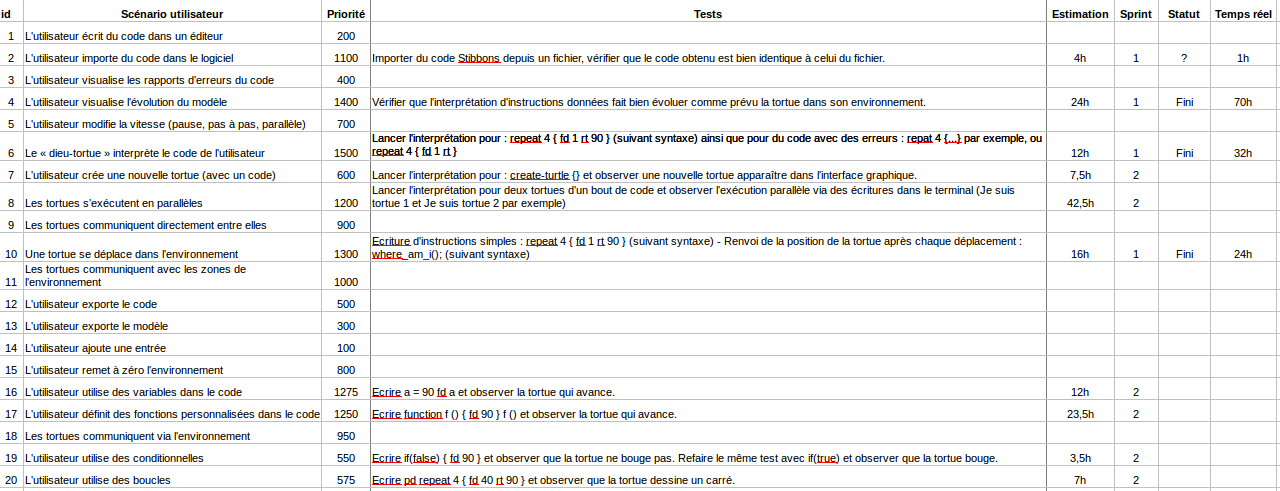
\includegraphics[scale=0.35]{doc/report/uml/backlogv1.png}
\end{figure}
Le backlog est composé de fonctionnalités, qui ont un indice entre 1000 et 0 pour leur importance du rendu final.

 On écrit aussi une \enquote{user-storie} pour chaque fonctionnalité. Cela correspond au test que l'on fait passer au programme pour valider la fonctionnalité.


A chaque sprint, on décide des fonctionnalités qu'on ajoute, et du nombre d'heures qu'on estime devoir y passer.


Voici pour comparer le backlog lors du début du sprint 4~\ref{backlogsp4} page~\pageref{backlogsp4} :


\begin{figure}[h]
\caption{\label{backlogsp4} Backlog sprint 4}
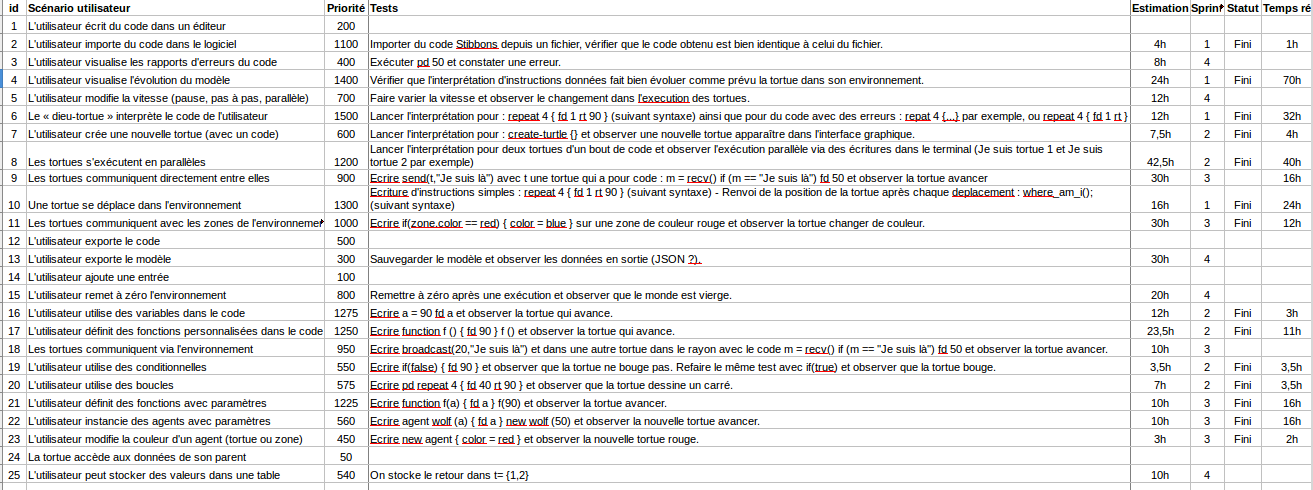
\includegraphics[scale=0.35]{doc/report/uml/backlogsp4.png}
\end{figure}
A la fin d'un sprint, on estime le temps passer sur chaque tâche, on fait le point sur notre avancée dans le projet.

Ici, on peut voir un ajout de fonctionnalités, le changement de statut des fonctionnalités réalisées, et le temps réel passer à les rendre utilisables.
Globalement, nous étions toujours dans les temps, car nous surestimions certaines tâches, qui s'averait plus facile que prévue.




\subsection{Git}
Git est hébergeur de code, de projet, qui permet d'avoir accès à ceux-ci n'importe où il y a internet.
Il s'utilise avec des systèmes de branches et s'utilise à la le plus souvent console, mais nous l'avons utiliser aussi avec Gitg, qui est une interface qui permet d'avoir un visuel des branches (Voir ~\ref{gitg} page~\pageref{gitg}).


\begin{figure}[h]
\caption{\label{gitg} Capture de Gitg}
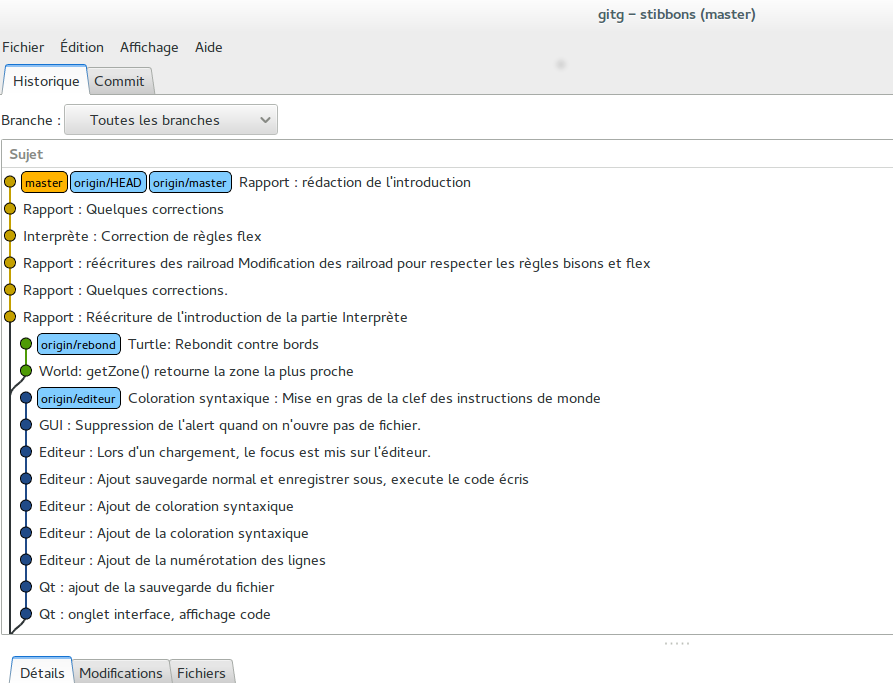
\includegraphics[scale=0.35]{doc/report/uml/gitbranche.png}
\end{figure}


Les commandes commence toujours par git :
\begin{itemize}
\item git checkout nom-branche, permet de changer de branche,
\item git branch, de savoir sur quel branche on est,
\item git add fichiers, permet de suivre des fichiers (enregistrer les modifications qu'on fait sur des fichiers),
\item git commit, permet de commiter les changements des fichiers qu'on suit,
\end{itemize}


De plus, Git permet sur son site de déclarer des \enquote{issues}. Ce sont des problèmes à corriger.



\subsection{Make}

Make est un utilitaire de construction de fichiers qui nous a été utile tout au long du projet pour construire les applications (stibbons et stibbons-cli), les tests unitaires, ou encore la documentation \LaTeX du projet. Il est également utile à l'installation des applications.

Il fonctionne en laissant l'utilisateur définir des règles de construction de fichiers, en listant les fichiers dont sa construction dépend et en définissant les commandes nécessaires à sa construction.

Make est alors appelé à construire une cible (un fichier ou non), construisant son arbre de dépendances, vérifiant l'existance de ces dernières, les construisant ou reconstruisant au besoin. Ainsi Make permet d'éviter les compilations ou recompilations inutiles, accélerant et automatisant la construction de logiciels ou de documents.
